\documentclass[12pt]{article}
\usepackage[margin=0.5in]{geometry} 
\usepackage{amsmath,amsthm,amssymb,amsfonts, enumitem, fancyhdr, color, comment, graphicx, environ}
\usepackage{course}
\usepackage{cse468-Spring22}
\usepackage{program}
\usepackage{fancybox}
\usepackage{adjustbox}
\usepackage{quantikz}
\usepackage{../bbkey}
\def\SquareOutline{%
\path (0,0) rectangle (1,1);%
}%
\def\Gate#1{\mbox{\textbf{#1}}}
\def\X{\Gate{X}}
\def\Z{\Gate{Z}}
\def\I{\Gate{I}}
\def\H{\Gate{H}}
\def\QZero{\ket{0}}
\def\QState#1{\ensuremath{\psi_{#1}}}

\def\Obox#1{\Ovalbox{\hbox to 1ex{\vrule width 0pt height 1ex\hss #1\hss}}}
\def\TFMarked#1#2{\ \stackbox[l][m]{\Obox{#1}~\textbf{true}\\\Obox{#2}~\textbf{false}}}
\def\TF{\TFMarked{\relax}{\relax}}
\def\exp#1{\ensuremath{e^{#1}}}
\newcommand{\Blank}[1][1in]{\mbox{\vrule width #1 depth 2pt}\vrule width 0pt height 2.0em}
\def\BlQb{\mbox{\ensuremath{\Blank[4em]\ket{0}+\Blank[4em]\ket{1}}}}
\newcommand{\Blanket}[1][3em]{%
\mbox{\ensuremath{|\,\Blank[#1]\,\rangle}}}

\def\Tall{\vrule width 0pt height 2em depth 0.5em}

\def\SQB#1#2{%
\ensuremath{%
\begin{pmatrix*}[r] #1 \\ #2\end{pmatrix*}}}

\def\SQBB{\SQB{\Blank[2em]}{\Blank[2em]}}

\def\DQB#1#2#3#4{%
\ensuremath{%
\begin{pmatrix*}[r] #1 \\ #2 \\ #3 \\ #4\end{pmatrix*}}}
\def\DQBB{\DQB{\Blank[2em]}{\Blank[2em]}{\Blank[2em]}{\Blank[2em]}}

\def\FactorProof{%
\begin{align*}
\SQB{a}{b} \otimes \SQB{c}{d} &= \DQBB{} \mbox{ (copy this from your \QState{2} answer top of page)}\\
a\cdot c &= \Blank[3em] \\
a\cdot d &= \Blank[3em] \\
b\cdot c &= \Blank[3em] \\
b\cdot d &= \Blank[3em]
\end{align*}
What is the contradiction, if any?
\LeaveSpace{2in}
}

\begin{document}

\begin{assignment}{Exam II}{27 April 2022}{End of class}

{\small {\large \fbox{READ THIS before starting!}}
This exam is open-book, open-notes, open-Internet, but you must do this
work on your own without contact or conversations with any person.
Because this exam is given in a somewhat distributed manner, no questions will be answered, and no clarifications will be given.  State your assumptions and count on us to be fair and flexible, especially if we have been unclear.


Your work must be legible.  Work that is
difficult to read will receive no credit.  There is a blank page at the end
if you want to show extra work there.

There are 118 points available for this exam, but it will only be scored out of 100.  Extra points earned here will count toward your total exam grade, including Exam~II.

You must sign the pledge below for your exam to count.  Any cheating will
cause the students involved to receive an F for this course. Other unpleasant
actions
may be taken.

You must fill in your identifying information correctly.  
}

\begin{center}\large
\begin{tabular}{|c|c|c|} \hline
\multicolumn{3}{|c|}{{\bf Print  clearly} the following information:}  \\ \hline
\multicolumn{3}{|l|}{Name (print clearly):\Tall{}\hbox to 3in{\hss}}  \\ \hline
\multicolumn{3}{|l|}{Student 6-digit ID (print {\it really} clearly):\Tall{}\hbox to 3in{\hss}} \\ \hline
\end{tabular}
\end{center}

{\bf Pledge:} On my honor, I have neither
given nor received any unauthorized aid on this exam.

Signed:  \Blank\Blank\Blank\Blank \\ \hbox to 5em{\hss}(Be 
sure you filled in your information in the box above!)
%
%
%
\clearpage
\begin{enumerate}
\item\Points{30} For the \textbf{true}/\textbf{false} questions below, indicate your response by marking an~\textbf{x} in the appropriate box, like this:
\TFMarked{\textbf{x}}{\relax} or \TFMarked{\relax}{\textbf{x}}.  

Each response is worth~3 points. You can miss any two responses and still get full credit for this portion.
\begin{itemize}
    \item Every unitary matrix has an inverse, which is that matrix's conjugate transpose.~\TF{}
    \item The states $\alpha\ket{0}+\beta\ket{1}$ and $\alpha\ket{0}-\beta\ket{1}$ differ only by a global phase.~\TF{}
    \item The states $\alpha\ket{0}-\beta\ket{1}$ and $-\alpha\ket{0}+\beta\ket{1}$ differ only by a global phase.~\TF{}
    \item The states $i\SQB{0}{1}$ and $\SQB{0}{-i}$ differ only by a global phase.~\TF{}
    \item Consider a state $\QState{}=\alpha\ket{0}+\beta\ket{1}$, and let $\QState{}^{\star}$ denote the conjugate transpose of \QState{}.   Then $\QState{}^{\star}\times\QState{}=0$.~\TF{}
    \item The conjugate transpose of \SQB{1}{i} is $\left(1\ \  i\right)$.~\TF{}
    \item The actions of any sequence of unitary gates applied to a single qubit can be represented by a single, unitary matrix.~\TF{}
    \item If the gate $A$ is applied to $\QState{}$ and the resulting state is then processed by gate $B$, the result is $A(B(\QState{}))$~\TF{}
    \item For the Pauli matrices, $\Gate{X}\Gate{Y}\Gate{Z}\Gate{Z}\Gate{Y}=\Gate{X}$~\TF{}
    \item The column vector for representing the state of an $n$-qubit system has $n$ entries.~\TF{}
    \item Given the state $\frac{\ket{00}+\ket{11}}{\sqrt{2}}$, measuring either qubit determines the value of the other qubit.~\TF{}
    \item The state $\frac{\ket{01}+\ket{10}}{\sqrt{2}}$ is an entangled state.~\TF{}
\end{itemize}

\clearpage\item\Points{30} For each question below, fill in the blank.  Your answer must appear in the provided blank for proper credit.  Write each response in the provided blank space, fully above the dark line.  For example, to express $\frac{i}{\sqrt{3}}$ you would write \Blank{}\hbox to 0pt{\hskip -4em\raisebox{4pt}{$i/\sqrt{3}$}\hss}.  


\begin{itemize}
    \item Consider the oracle portion of a circuit below for an $8$-bit instance of the Bernstein--Vazirani problem.  Recall the oracle computes $y=x\oplus s$ for a secret bit vector~$s$.
    
    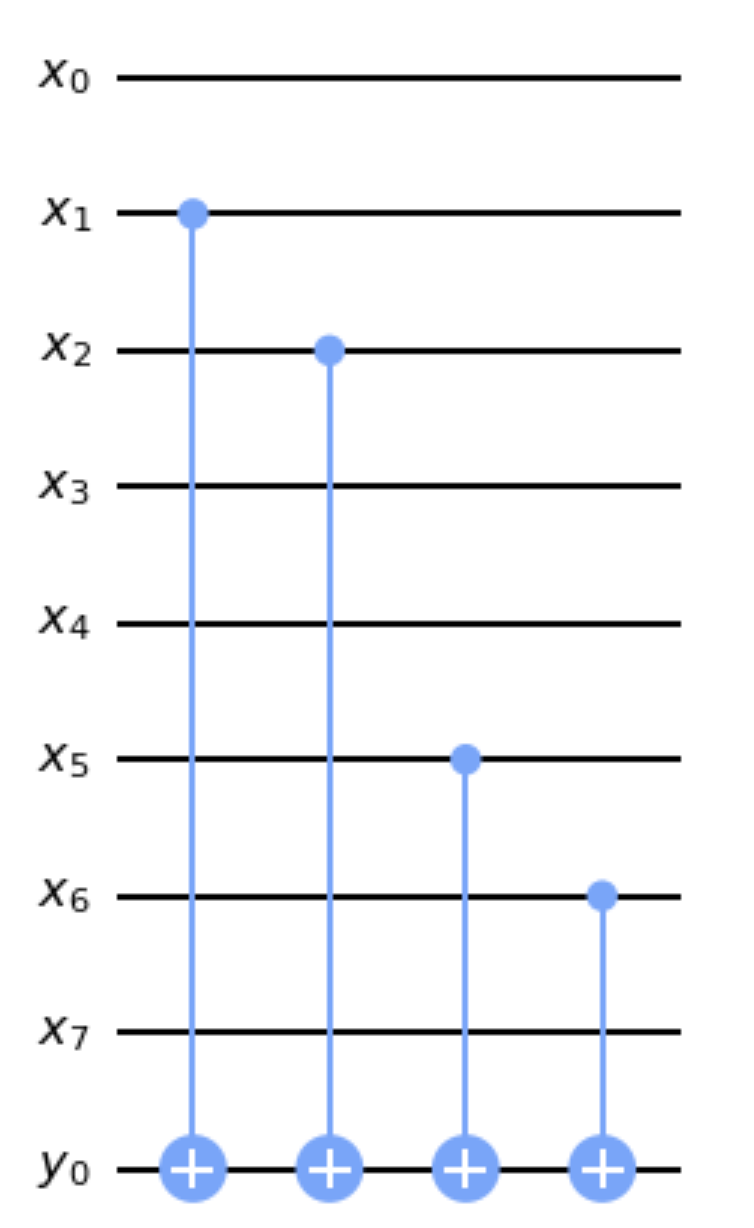
\includegraphics[scale=0.4]{bv.png}
    
    What is the secret $s$ here? \Blank[2in]{}
    \item If this oracle is used in the complete Deutsch--Jozsa algorithm, what possible amplitude(s) can be measured on $\ket{00000000}$?
    
    \Blank[4in]{}
    \item What other computational basis vector(s), if any, will have non-zero amplitude for Deutsch--Jozsa if the above oracleis used?  
    
    \Blank[4in]{}
\end{itemize}

\clearpage\item\Points{20}

Consider the circuit below where some arbitrary single-qubit gate $U$ acts on the top qubit.  Following that, a CNOT gate is applied from the top to the bottom qubit:

\adjustbox{valign=t}{\begin{quantikz}
\lstick{$\ket{0}$} &  \gate{U}& \ctrl{1} & \qw & \gate{?} & \qw \\
\lstick{$\ket{0}$} &   \qw  & \targ{} & \qw &\qw& \qw
\end{quantikz}}

While we know general cloning of a quantum state is impossible, there are exactly two states resulting from $U\ket{0}$ that are successfully cloned onto the bottom qubit using the above circuit.

Those states are \Blank{} and \Blank{}.

If we wanted to restore the top qubit to its state prior to applying $U$, what gate would we place in the ``?'' box? \Blank{}

The algorithm we studied for phase estimation applies gates and measures the qubits of a quantum system, thus transforming and then collapsing each qubit's state.

Based on the above and on your knowledge of how phase estimation is performed, describe how we could perform phase estimation on an $n$-qubit system, but now with $n$~ancillary (extra, additional) qubits, and now restoring the $n$ primary bits to their state prior to the actions performed for phase estimation.
\clearpage\item\Points{20}
%%%
%%%



Fill in the column vectors to show your analysis of the states at the indicated positions of the circuit.  The rest of this page is scratch space:  \textbf{the parts to fill in are on the next page}.
\Continued{}

$\ket{\QState{0}}=\DQBB{}$  $\ket{\QState{1}}=\DQBB{}$  $\ket{\QState{2}}=\DQBB{}$

\item Either Express \ket{\QState{2}} as the product of two 1-quibit states:

\[\ket{\QState{2}} = \SQBB \otimes \SQBB \]
or complete the proof below to show that it cannot be factored:
\FactorProof{}

%%%
%%%





\clearpage\item\Points{10} Bloch Sphere Orienteering:  all answers are in the standard basis.  Write each amplitude in the provided blank space, fully above the dark line.  For example, to express $\frac{i}{\sqrt{3}}$ you would write \Blank{}\hbox to 0pt{\hskip -4em\raisebox{4pt}{$i/\sqrt{3}$}\hss}.

Each response is worth 1 point.



\begin{itemize}
    \item We begin at the North pole of the Bloch sphere.
    \item We are in state \BlQb{}.
    \item We experience a \Gate{Y} gate.  We are now at \BlQb{}.
    \item We return to the North pole.
    \item We experience an \H{} gate.  We are now at \BlQb{}.
    \item We then experience a \Z{} gate.  We are now at state \BlQb{}.
    \item We finally experience an \H{} gate.  We are now at state \BlQb{}.
\end{itemize}

\clearpage\item\Points{10}  Suppose Alice and Bob decide to form a shared key using the BB84 protocol.  The table below shows the bases they will publish along with their observed results.   Recall the correspondence between observed quantum state and bit values:
\begin{BBKey}
\begin{center}
\BBBasis{}
\end{center}
\end{BBKey}
\def\RowU#1#2#3#4{%
\vrule width 0pt depth 0.5em height 1.2em#1 &#2 & #3 & #4 & & & {\vrule width 0pt depth 13pt\small\TF{}}  \\ \hline}
\def\Row#1#2#3{%
\RowU{\STD}{#1}{#2}{#3}}
\def\RowX#1#2#3{%
\RowU{\HDM}{#1}{#2}{#3}}

Fill in the table below and be sure to put your final answer for grading in the space provided at the bottom of this page.  Note the following:
\begin{description}
  \item[Agreed Bit?]  After publishing their list of bases, what bit (0 or 1), \textbf{IF ANY}, would Alice and Bob each believe they share, assuming they do not believe Eve is present.
  \item[Eve Detected?] Does this particular row allow detection of Eve if Alice's and Bob's bits from this row are published?
\end{description}

\begin{BBKey}
\begin{center}\Large
\begin{tabular}{c|c||c|c||c|c||c}
\multicolumn{2}{c||}{Alice Sends} & \multicolumn{2}{c||}{Bob Receives}& \multicolumn{2}{c||}{Agreed bit?}&Eve \\
Basis & Obs & Basis & Obs & Alice & Bob & Detected?\\\hline
\Row{\BBRt}{\STD}{\BBRt}
\Row{\BBUp}{\STD}{\BBUp}
\Row{\BBRt}{\STD}{\BBRt}
\Row{\BBUp}{\HDM}{\BBNe}
\Row{\BBRt}{\HDM}{\BBSe}
\RowX{\BBNe}{\HDM}{\BBSe}
\RowX{\BBSe}{\HDM}{\BBSe}
\RowX{\BBNe}{\HDM}{\BBNe}
\RowX{\BBNe}{\HDM}{\BBNe}

\end{tabular}
\end{center}
\end{BBKey}
\begin{itemize}
    \item Alice believes the shared key is~\Blank[4in]{}
    \item Bob believes the shared key is\ \ ~\Blank[4in]{}
    \item Eve could have been detected in how many rows of your table?~\Blank{}
\end{itemize}

\clearpage\item\Points{10}
Consider the following entangled state of three qubits:
\[\frac{\ket{000}+\ket{111}}{\sqrt{2}}\]
In lecture we studied how to entangle that third qubit with the first two.  In this problem we consider \emph{disentangling} the third qubit from the first two, without resorting to measurement.

Recall that we entangle the third new qubit $q_{3}$ with those that came before ($q_{1}, q_{2}$) using a \Gate{CNOT} gate, controlled by either $q_{1}$ or $q_{2}$, and applied to $q_{3}$ which is initialized to~\ket{0}.  Because \Gate{CNOT} is its own inverse, we try using the gate again to disentangle~$q_{3}$.
\begin{enumerate}
  \item\Points{2} 
  \[(\I\otimes\Gate{CNOT})(\ket{000}) = \Blanket{}\]
\item\Points{2} 
  \[(\I\otimes\Gate{CNOT})(\ket{111} = \Blanket{}\]
\item \Points{3} By linearity,
\[(\I\otimes\Gate{CNOT})\left(\frac{\ket{000}+\ket{111}}{\sqrt{2}}\right) = \frac{\Blank[4em]+\Blank[4em]}{\sqrt{2}} = \frac{\ket{00}+\ket{11}}{\sqrt{2}} \otimes \Blanket{}\]
\item \Points{2} Qubit $q_3$ is now disentangled and in its current state it measures as~$\Blanket{}$.
\item \Points{1} Measuring $q_3$ causes collapse of the other two qubits? \TF{}

\end{enumerate}

\end{enumerate}

\end{assignment}
\Bpage{}

\end{document}
